\section{Hardware}
  Für die technische Umsetzung werden eine Reihe von Komponenten verwendet.

  \subsection{Raspberry Pi 3}
  
    % image of the raspberry pi - source: http://www.raspberrypi.org
    \begin{minipage}{\columnwidth}
      \makeatletter
      \def\@captype{figure}
      \makeatother
      \centering
      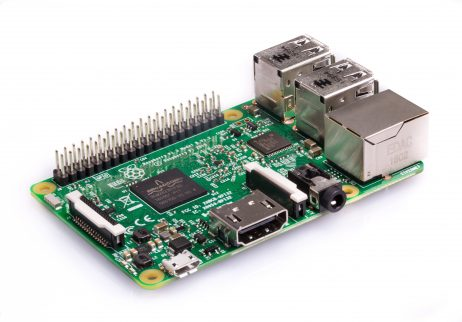
\includegraphics[width=0.6\linewidth]{images/hw_raspberrypi3.jpg}
      \caption{Raspberry Pi 3 Model B}
      \label{fig:img-hw-01}
    \end{minipage}
    \vspace{0.5cm}
    Das Herzstück des Projekts bildet ein Raspberry Pi 3 Model B. Ausgestattet
    ist dieser Mini-PC neben den üblichen Schnittstellen mit einem Wifi Modul
    und verfügt

  \subsection{Motorcontroller}

    % image of the motor and servo controller module  - source: https://www.makerlab-electronics.com
    \begin{minipage}{\columnwidth}
      \makeatletter
      \def\@captype{figure}
      \makeatother
      \centering
      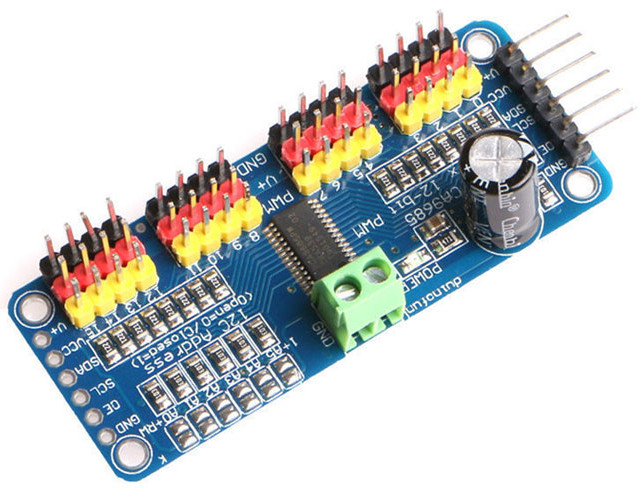
\includegraphics[width=0.6\linewidth]{images/hw_pca9685.jpg}
      \caption{PCA9685 Controller Modul}
      \label{fig:img-hw-02}
    \end{minipage}
    \vspace{0.5cm}

  \subsection{Ultraschallsensor}

    % image of ultrasonic sensor module  - source: https://www.makerfabs.com 
    \begin{figure}[H]
    \center
    \begin{subfigure}{.5\textwidth}
      \centering
      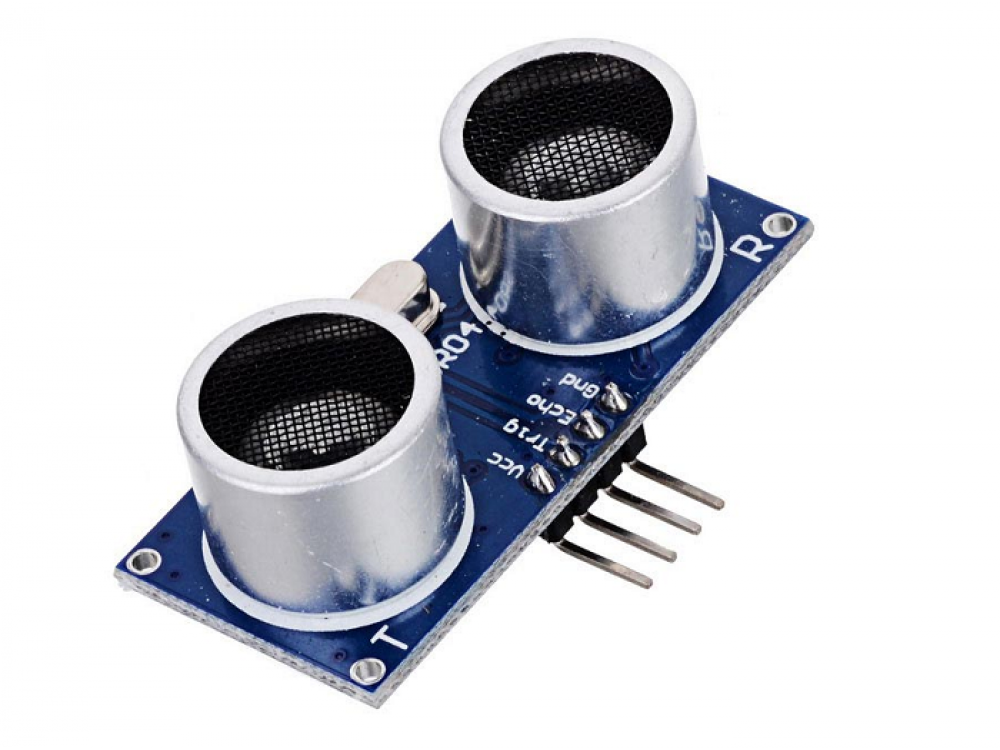
\includegraphics[width=.8\linewidth]{images/hw_hcsr04_01.png}
    \end{subfigure}%
    \begin{subfigure}{.5\textwidth}
      \centering
      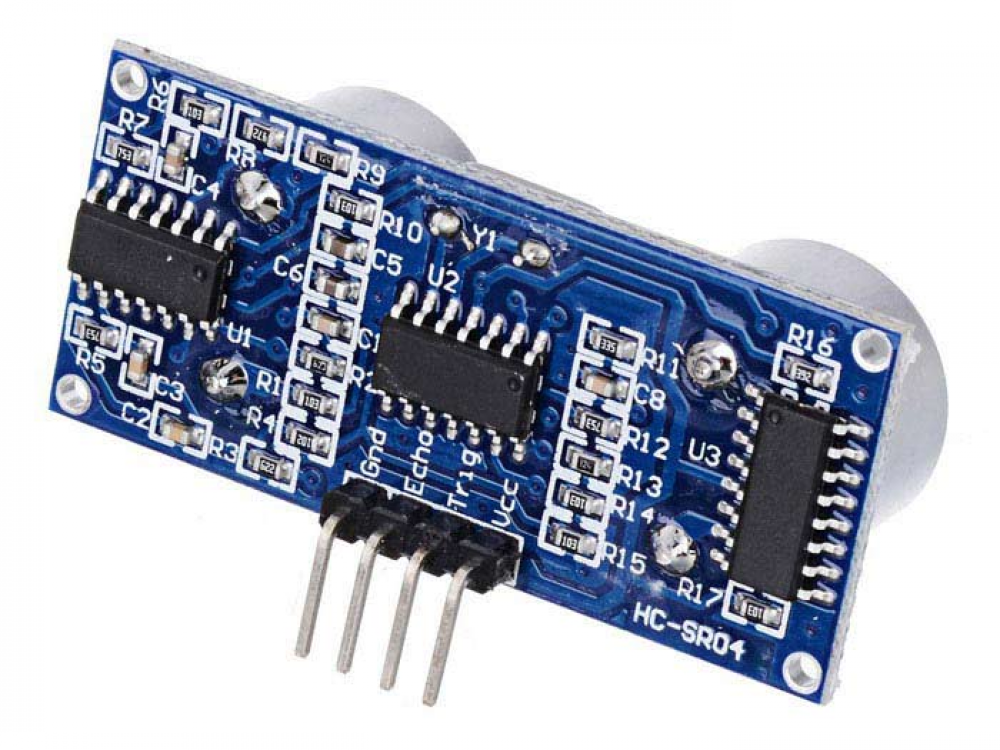
\includegraphics[width=.8\linewidth]{images/hw_hcsr04_02.png}
    \end{subfigure}
      \caption{HC-SR04 Sensor Modul}
      \label{fig:img-hw-03}
    \end{figure}
    \vspace{0.5cm}

  \subsection{RC Fahrzeug}

    Ein RC Fahrzeug von Conrad ist auch verwendet worden, keine Ahnung, was das
    genau für eins war...
    \ \\
